\documentclass[a4paper,14pt]{article}

\usepackage{comment} % Para comentar várias linhas ao mesmo tempo

%matemática
\usepackage{amsmath}
\usepackage{amssymb}

%diagramação
\usepackage{extsizes}
\everymath{\displaystyle}
\usepackage{geometry}
\usepackage{fancyhdr}
\usepackage{multicol}
\usepackage{graphicx}
\usepackage[brazil]{babel}
\usepackage[shortlabels]{enumitem}
\usepackage{cancel}
\usepackage{textcomp}
\usepackage{tcolorbox}

%tabelas
\usepackage{array} % Para melhor formatação de tabelas
\usepackage{longtable}
\usepackage{booktabs}  % Para linhas horizontais mais bonitas
\usepackage{float}   % Para usar o modificador [H]
\usepackage{caption} % Para usar legendas em tabelas
\usepackage{wrapfig} % Para usar tabelas e figuras flutuantes
\usepackage{xcolor} % Para cores do fundo de tabelas
\usepackage{colortbl} % Para cores do fundo de tabelas

%tikzpicture
\begin{comment}
	\usepackage{tikz}
	\usepackage{scalerel}
	\usepackage{pict2e}
	\usepackage{tkz-euclide}
	\usetikzlibrary{calc}
	\usetikzlibrary{patterns,arrows.meta}
	\usetikzlibrary{shadows}
	\usetikzlibrary{external}
\end{comment}


%pgfplots
\usepackage{pgfplots}
\pgfplotsset{compat=newest}
\usepgfplotslibrary{statistics}
\usepgfplotslibrary{fillbetween}

%colours
\usepackage{xcolor}



\columnsep=2cm
\hoffset=0cm
\textwidth=8cm
\setlength{\columnseprule}{.1pt}
\setlength{\columnsep}{2cm}
\renewcommand{\headrulewidth}{0pt}
\geometry{top=1in, bottom=1in, left=0.7in, right=0.5in}

\pagestyle{fancy}
\fancyhf{}
\fancyfoot[C]{\thepage}

\begin{document}
	
	\noindent\textbf{6FMA123 - Matemática} 
	
	\begin{center}Casos de congruência de triângulos (Versão estudante)
	\end{center}
	
	\noindent\textbf{Nome:} \underline{\hspace{10cm}}
	\noindent\textbf{Data:} \underline{\hspace{4cm}}
	
	%\section*{Questões de Matemática}
	
	\begin{multicols}{2}
	    \noindent Casos de congruência de triângulos:
	    \begin{itemize}
	    	\item lado, ângulo, lado (LAL);
	    	\item lado, lado, lado (LLL);
	    	\item ângulo, lado, ângulo (ALA).
	    \end{itemize}
	    Mediatriz de um segmento é a reta que passa pelo seu ponto médio formando 90°.
		\noindent\textsubscript{--------------------------------------------------------------------------}
		\begin{enumerate} 
			\item Aponte, nas figuras a seguir, o par de triângulos congruentes. (Os triângulos foram mal desenhados de propósito.)
			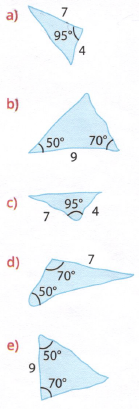
\includegraphics[width=1\linewidth]{6FMA123_imagens/imagem1}
			\item Observe a figura a seguir, em que $m$ é a mediatriz de $\overline{AB}$.
			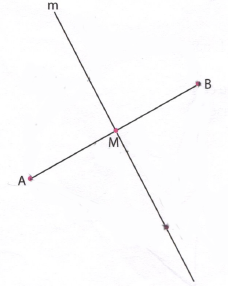
\includegraphics[width=1\linewidth]{6FMA123_imagens/imagem2}
			\begin{enumerate}[a)]
				\item Traçando os segmentos $\overline{AX}$ e $\overline{BX}$ no desenho anterior, você obterá os triângulos $AMX$ e $BMX$. Prove que $\Delta$$AMX \cong \Delta$$BMX$, justificando sua resposta. \\\\\\\\\\\\\\\\\\\\ 
				\item O que você pode afirmar sobre as distâncias de $AX$ e $BX$? \\\\\\\\
				\item Toda reta é um conjunto de pontos. Observando o que acontece com o ponto $X$, escolhido ao acaso na reta $m$, é possível tirar uma conclusão a respeito de todos esses pontos. Que conclusão seria essa? Como você descreveria a mediatriz $m$ do segmento $\overline{AB}$, com base nessa conclusão? \newpage
			\end{enumerate}
			\item Usando seus instrumentos de desenho, construa triângulos cujos lados são congruentes aos segmentos dados a seguir. \\
			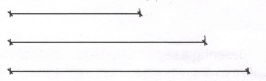
\includegraphics[width=1\linewidth]{6FMA123_imagens/imagem3} \\\\\\\\\\\\\\\\\\\\\\\\\\\\\\\\\\\\\\\\\\\\\\\\\\\\\\\\\\\\\\\\
			\item Na figura a seguir, $AC = AD$.
			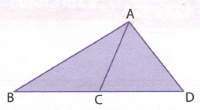
\includegraphics[width=1\linewidth]{6FMA123_imagens/imagem4}
			É verdade que $ABC$ e $ABD$ são congruentes? Justifique. \newpage
			%49 a 53
			\item Triângulos retângulos são aqueles que têm um ângulo reto. No triângulo retângulo, os dois lados menores recebem o nome de \textbf{catetos} e o lado maior é chamado de \textbf{hipotenusa}. Podemos afirmar que dois triângulos retângulos são congruentes quando os dois têm catetos de medida $a$ e $b$, em que $a$ e $b$ podem ser diferentes. Justifique essa afirmação. \\
			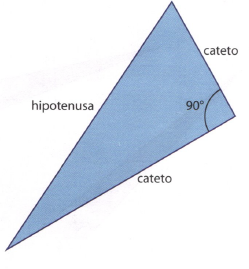
\includegraphics[width=1\linewidth]{6FMA123_imagens/imagem5}
			\\\\\\\\\\\\\\\\\\\\\\\\\\\\\\
			\item \begin{enumerate}[a)]
				\item Copie os dois pontos desenhados a seguir em seu caderno de desenho. Usando régua e compasso, ache um ponto que está a distância de 3 cm de ambos os pontos. \\
				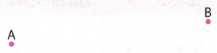
\includegraphics[width=1\linewidth]{6FMA123_imagens/imagem6}
			\end{enumerate}
			\item Em cada item há um par de triângulos congruentes. Indique o caso de congruência e determine o valor de $x$ (medida de comprimento ou de ângulo).\\
			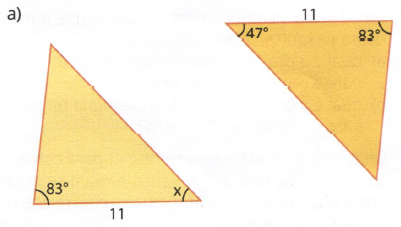
\includegraphics[width=1\linewidth]{6FMA123_imagens/imagem7}\\
			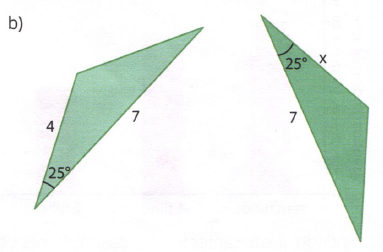
\includegraphics[width=1\linewidth]{6FMA123_imagens/imagem8}\\
			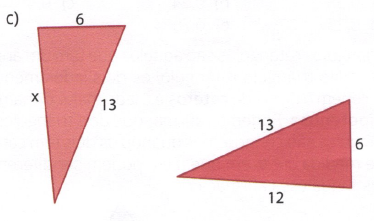
\includegraphics[width=1\linewidth]{6FMA123_imagens/imagem9}\\
			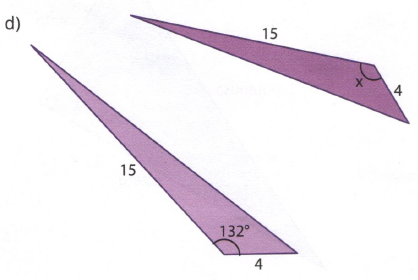
\includegraphics[width=1\linewidth]{6FMA123_imagens/imagem10}\\
			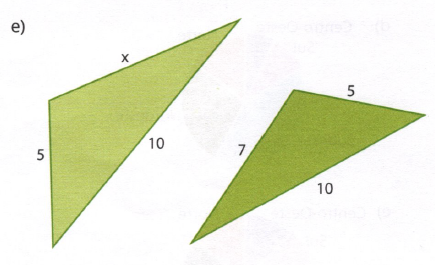
\includegraphics[width=1\linewidth]{6FMA123_imagens/imagem11}\\
			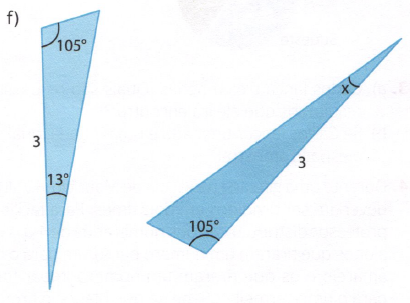
\includegraphics[width=1\linewidth]{6FMA123_imagens/imagem12} \\
			\item A seguir, temos $AE = AD, \overline{AB} \perp \overline{EC}$ e $\overline{BD} \perp \overline{AC}$. Prove que $\hat{B} \cong \hat{C}$.\\
			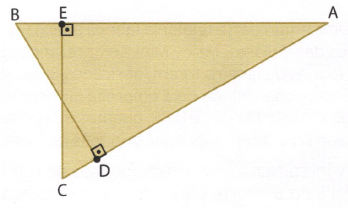
\includegraphics[width=1\linewidth]{6FMA123_imagens/imagem13} \\\\\\\\\\
			\item O desenho a seguir se refere ao retângulo de vértices $A, B, C$ e $D$. O segmento $\overline{AC}$ é uma diagonal do retângulo. Mostre que os dois triângulos assim formados são congruentes, baseando-se em um dos critérios já vistos, LAL ou LLL. \\
			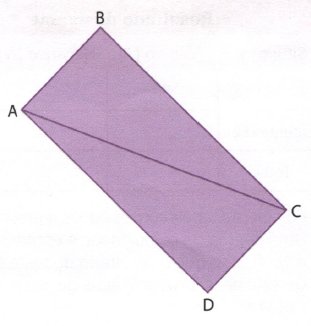
\includegraphics[width=1\linewidth]{6FMA123_imagens/imagem14} \\ 
		\end{enumerate}
		$~$ \\ $~$ \\ $~$ \\ $~$ \\ $~$ \\ $~$ \\ $~$ \\ $~$ \\ $~$ \\ $~$ \\ $~$ \\ $~$ \\ $~$ \\ $~$ \\ $~$ \\ $~$ \\ $~$ \\ $~$ \\ $~$
	\end{multicols}
\end{document}